\documentclass[border=10pt]{standalone}
\usepackage{tikz}\usepackage{amsmath}\usetikzlibrary{arrows.meta}
\begin{document}
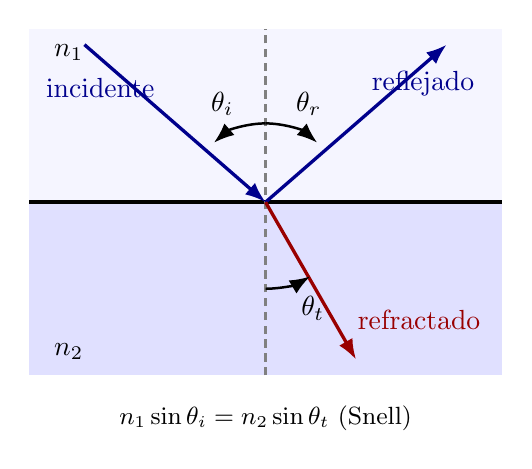
\begin{tikzpicture}[line width=0.9pt,>={Latex[length=2.6mm]}]
  \fill[blue!4] (-3,0) rectangle (3,2.2);
  \fill[blue!12] (-3,-2.2) rectangle (3,0);
  \draw[line width=1.2pt] (-3,0)--(3,0);
  \draw[densely dashed,gray] (0,-2.2)--(0,2.2);
  \node at (-2.5,1.9){$n_1$}; \node at (-2.5,-1.9){$n_2$};
  % incidente
  \draw[->,blue!55!black,line width=1.2pt] (-2.3,2.0)--(0,0);
  \node[blue!55!black] at (-2.1,1.45){incidente};
  % reflejado
  \draw[->,blue!55!black,line width=1.2pt] (0,0)--(2.3,2.0);
  \node[blue!55!black] at (2.0,1.5){reflejado};
  % refractado (mas cerca de la normal, n2>n1)
  \draw[->,red!60!black,line width=1.2pt] (0,0)--(1.15,-2.0);
  \node[red!60!black] at (1.95,-1.5){refractado};
  % angulos
  \draw[->] (0,1.0) arc (90:131:1.0); \node at (-0.55,1.25){$\theta_i$};
  \draw[->] (0,1.0) arc (90:49:1.0); \node at (0.55,1.25){$\theta_r$};
  \draw[->] (0,-1.1) arc (270:301:1.1); \node at (0.6,-1.35){$\theta_t$};
  \node at (0,-2.75){\small $n_1\sin\theta_i=n_2\sin\theta_t$ (Snell)};
\end{tikzpicture}
\end{document}
